%----------------------------------------------------------------------------
%----------------------------------------------------------------------------

\makeatletter\def\input@path{{./TexInputs/}}\makeatother

\documentclass{egpubl}
\usepackage{sca2014}

% --- for  EG Workshop Proceedings
\WsSubmission    % uncomment for submission to EG Workshop
%\WsPaper         % uncomment for final version of EG Workshop contribution
%
\electronicVersion % can be used both for the printed and electronic version

\PrintedOrElectronic

% \usepackage{t1enc,dfadobe} % produces upright Greek, which I think is ugly -- Rahul
\usepackage[T1]{fontenc}
\usepackage{mathptmx}

\usepackage{egweblnk}
\usepackage{cite}

% end of SCA format prologue

\usepackage{amsmath}
\usepackage{amssymb}
\usepackage{bm}
\usepackage{booktabs}
\usepackage{graphicx}
\usepackage{microtype}
\usepackage{url}
\usepackage{xspace}

\hypersetup{
  breaklinks,
  letterpaper,
  bookmarks,
  bookmarksnumbered,
  colorlinks,
  linkcolor=black,
  citecolor=black,
  urlcolor=black,
  pdfpagemode={UseThumbs}
}

\graphicspath{{Figures/}{TexInputs/}{images/}}
\urlstyle{sf}

%----------------------------------------------------------------------------
%----------------------------------------------------------------------------


\renewcommand{\vec}{\mathbf}
\newcommand{\tr}{^T}

\newcommand{\james}[1]{\textcolor{blue}{(#1 ---James)}}
\newcommand{\rahul}[1]{\textcolor{blue}{(#1 ---Rahul)}}
\newcommand{\woojong}[1]{\textcolor{magenta}{(#1 ---Woojong)}}

\renewcommand{\thefootnote}{\arabic{footnote}}

%----------------------------------------------------------------------------
%----------------------------------------------------------------------------


\newcommand{\theTitle}{View-Dependent Adaptive Cloth Simulation}

\title{\theTitle}

\author[W. Koh, R. Narain, \& J. F. O'Brien]{Woojong Koh\qquad Rahul Narain\qquad James F.
O'Brien\\ University of California, Berkeley}

\newcommand{\arcsim}{\textsc{Arc}Sim\xspace}

%----------------------------------------------------------------------------
%----------------------------------------------------------------------------

\begin{document}

\maketitle

\begin{abstract}
This paper describes a method for view-dependent cloth simulation using
dynamically adaptive mesh refinement and coarsening. Given a prescribed camera
motion, the method adjusts the criteria controlling refinement to account for
visibility and apparent size in the camera's view. Objectionable dynamic
artifacts are avoided by anticipative refinement and smoothed coarsening. This
approach preserves the appearance of detailed cloth throughout the animation
while avoiding the wasted effort of simulating details that would not be
discernible to the viewer. The computational savings realized by this method
increases as the scene complexity grows, producing a $2\times$ speed-up for a
single character and more than $4\times$ for a small group.

\begin{classification} % according to http://www.acm.org/class/1998/
 \CCScat{Computer Graphics}{I.3.5}{Computational Geometry and Object Modeling}{Physically based modeling};
 \CCScat{Computer Graphics}{I.3.7}{Three-Dimensional Graphics and Realism}{Animation};
 \CCScat{Simulation and Modeling}{I.6.8}{Types of Simulation}{Animation}.
\end{classification}

\end{abstract}

%----------------------------------------------------------------------------
%----------------------------------------------------------------------------

\hypersetup{
  pdftitle={\theTitle},
  pdfauthor={Submission ID 1011},
  pdfsubject={Submitted to SCA 2014.},  %<>
%  pdfkeywords={\theKeywords}  %<>
}


%----------------------------------------------------------------------------


\section{Introduction}

\begin{figure}[t]
    \centering
    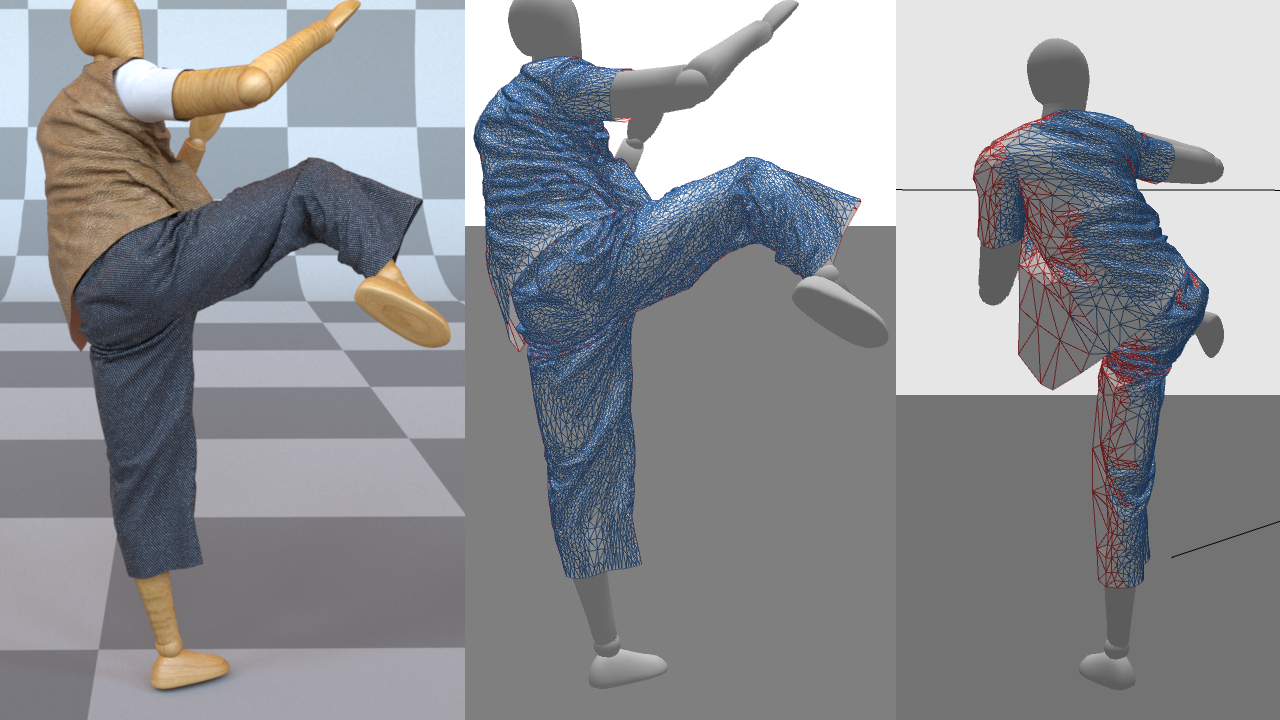
\includegraphics[width=1.0\columnwidth]{karate/karate}
	\vspace*{-.2in}
    \caption{The clothing on this character uses view-dependent simulation.  
	Visible areas (blue) are simulated at high resolution, as measured in screen-space.  
	Areas not visible to the camera (red) are simulated at reduced resolution.
    The first two images show views from the camera's perspective.  The rightmost image 
	shows an outside perspective with the camera's view frustum drawn in black wireframe. 
}
    \label{fig:teaser}
	\vspace*{-.2in}
\end{figure}

Cloth simulation for visual effects has reached a mature state where
the use of virtual characters wearing simulated clothing is now
widespread.  However, cloth simulation remains computationally
expensive, particularly when films require high-quality, realistic
results computed at high resolution.  For characters that are far from
the camera, or otherwise less visible in a shot, most fine details
will not be visible to the viewer and work spent computing those
details is wasted.  In most film production settings, both the camera
and character motion are known before the simulations are run, and one
could use this information to substitute cheaper low-resolution
simulations on distant or out-of-frame characters.  Unfortunately,
manually swapping some characters to low-resolution simulations is
cumbersome, particularly when a single character's clothing requires
high-resolution for some parts of a shot but not others, but the cloth
motion must appear coherent throughout.  For closeup shots where only
part of a character is in frame, savings could also be realized by reducing
the computation devoted to out-of-frame cloth, so long as such savings
don't result in dynamic artifacts that affect visible parts of the
cloth.

In this paper we describe a method for view-dependent simulation using
dynamically adaptive mesh refinement and coarsening.  Instead of using
a fixed-resolution simulation mesh, the mesh undergoes local
adaptation based on the geometric and dynamic detail of the simulated
cloth. The degree to which this detail is resolved is adjusted locally
based on the view of the simulated cloth.  Areas that appear large
in the camera will be refined to show finely detailed dynamics.  Areas
that are out of frame, facing away from the camera, or at a distance
will be correspondingly less refined.

The goal of this work is to preserve the appearance of detailed
simulation throughout the animation while avoiding the wasted effort
of simulating details that will not be apparent to the viewer.
Further, there should be no visible dynamic artifacts created due to
varying refinement as the camera and objects move about.  Finally,
cloth that leaves and reenters visibility should appear to have
coherent and consistent dynamics.

% \rahul{This paragraph is a little repetitive with paragraph 2.}
Our work builds on the publicly available \arcsim
framework (\url{http://graphics.berkeley.edu/resources/ARCSim}) which
can be used to animate sheets of deformable materials such as cloth, paper,
plastic, and metal. \arcsim adaptively refines anisotropic triangle meshes to
efficiently resolve the geometric and dynamic detail of the simulated objects.
Our method modifies the metrics used by \arcsim so that local mesh visibility
is accounted for during refinement. Given the existing framework for adaptivity,
our view-dependent refinement is easy to implement and has negligible overhead.

In cases where only a single character is being modeled, we realize modest savings of
roughly a $2.4\times$ speed-up in comparison with an adaptive simulation of \arcsim due to
coarsening out-of-view and back-facing parts of the character's clothing. For small crowd
scenes, the savings are larger, up to $4.5\times$, as background and out-of-view
characters are automatically coarsened. Compared to a non-adaptive simulation the speed-up
is more than $9\times$. For massive crowd scenes with thousands of agents, we expect that
even greater savings could be realized.



%----------------------------------------------------------------------------




\section{Related Work}

Adaptive discretizations have been found to give significant performance and
scalability benefits for a number of computationally intensive simulation
tasks. In fluid simulation, detailed liquid surfaces can be animated
efficiently by refining the spatial resolution near the surface using octrees
\cite{Losasso:2004:SWS}, adaptively sampled particles \cite{Adams:2007:ASP},
tall-cell grids \cite{Chentanez:2011:REW}, or tetrahedral meshes
\cite{Klingner:2006:FAD,Chentanez:2007:LSL,Ando:2013:HAL}. Adaptive refinement
and simplification techniques have also been proposed for mass-spring systems
\cite{Hutchinson:1996:ARM}, articulated bodies \cite{Redon:2005:ADA} and
finite element models \cite{Grinspun:2002:CSF}. Most relevant to our work
are techniques for adaptive cloth simulation
\cite{Thingvold:1990:PMB,Li:2005:CAA,Villard:2005:AMC,Brochu:2012:EGE,Narain:2012:AAR},
which use remeshing to resolve detailed wrinkles and folds. The approach of
Narain et al. \cite{Narain:2012:AAR} has also been extended to efficiently model
plastic deformation and sharp creases \cite{Narain:2013:FCA} as well as complex
fracture patterns \cite{Pfaff:2014:ATC}. However, all the techniques described
above are view-independent and rely only on geometrical and dynamical
properties of the simulated system.

For animation applications, a number of techniques have also been proposed that
take into account the current viewpoint and attempt to expend less
computational effort in regions that are visually less important. One approach,
known as simulation level of detail, is to switch between dynamical
models of varying degrees of simplification, depending on the viewpoint.
Carlson and Hodgins \cite{Carlson:1997:SLD} introduced such a method for
real-time animation of large groups of legged creatures. Their
approach required the user to manually design the simplified models for each
level of detail, whereas ours does not.  Subsequent work has sought to generate approximated
models automatically, for example for particle systems~\cite{OBrien:2001:ASP},
plants~\cite{Beaudoin:2004:SLD}, and hair~\cite{Ward:2003:MHU}.

Alternatively, one can modify the simulation resolution based on the viewpoint without changing the underlying model.
Barran \cite{Barran:2006:VDF} performed fluid simulation on a non-Cartesian grid based on cylindrical coordinates centered at the viewer, thus directly taking the distance from the viewer into account in the
discretization.
Viewpoint information has also been used to vary simulation resolution in traditional adaptive discretizations for fluids, such as octrees \cite{Kim:2006:VAA,Bunlutangtum:2011:EVA} and adaptive particles \cite{Solenthaler:2011:TPS}.

In our work, we also take inspiration from geometric level of detail techniques, such as those for real-time rendering of terrain~\cite{Duchaineau:1997:RTR,Hoppe:1998:SVL} or complex scenes like architectural walkthroughs~\cite{Funkhouser:1993:ADA}.
These techniques inform our understanding of the important view-dependent criteria for representing geometrical detail.
Hoppe~\cite{Hoppe:1997:VRP} used surface orientation and screen-space geometric
error as refinement criteria.
Xia et al.~\cite{Xia:1997:ARL} further propose the use of local illumination gradients, projected lengths of edges in screen space, and silhouette boundaries.

%----------------------------------------------------------------------------

\section{Method}

Our view-dependent adaptive remeshing scheme builds on the adaptive anisotropic
remeshing framework described by Narain et al.~\cite{Narain:2012:AAR}. We introduce a new
view-dependent refinement strategy that complements their use of dynamical and
geometrical refinement criteria. This approach realizes significant speed
improvements by extending the domain of adaptive remeshing to include
perceptual properties as well as physical ones.

The method of Narain et al.~defines a \emph{sizing field} that specifies
the desired spatially varying resolution of the simulation mesh, taking into account various geometric and dynamic criteria such as local
curvature, velocity gradient, compressive strain, and obstacle proximity. It is
represented as a $2 \times 2$ symmetric tensor field $\mathbf{M}$ which is first computed on faces and then transferred to vertices via area-weighted averaging.
Once the sizing field is defined, an edge between
vertices $i$ and $j$ is considered valid if its size with respect to $\mathbf
M$,
\begin{equation} \label{eq:invalid}
    s(i, j)^2 = \mathbf{u}^{\mathsf T}_{ij} \left( \frac{\mathbf{M}_i + \mathbf{M}_j}{2} \right) \mathbf{u}_{ij},
\end{equation}
does not exceed $1$, where $\mathbf{u}_{ij} = \mathbf u_i - \mathbf u_j$ is the
vector between the two vertices in material space. If $s(i,j)^2 > 1$, the edge
is deemed invalid and must be split.
The remeshing algorithm proceeds by splitting all invalid edges, collapsing as many edges as possible without introducing new invalid edges, and flipping edges to maintain an anisotropically Delaunay triangulation.
This procedure produces a mesh that is as coarse as possible while containing no invalid edges and remaining Delaunay in the anisotropic space of the metric.


We modify their algorithm so that, rather than using purely physical and geometrical criteria to determine the mesh resolution,
we vary the desired degree of refinement over space and time based on visual importance relative to a
specified camera motion.
We implement this variation by modifying the sizing field $\mathbf{M}$ so that
the size of each face is no more than what is needed to resolve visually
important features.
 This modification reduces computational effort in regions
that are less visible from the camera, bringing about a more efficient simulation without losing significant visual detail.


Our implementation considers two visibility criteria. In regions that are
not visible from the current camera position, that is, those that are out of
frame or facing away from the camera, we scale the sizing field to uniformly
coarsen the mesh. In regions that are visible, we control the sizes of elements
in terms of their projected lengths in screen space so that distant or foreshortened elements are coarser. This
approach is roughly equivalent to adaptivity based on screen-space metrics.
However, to avoid artifacts that would occur due to fast-moving cameras or cuts
between views, our algorithm applies conservative spatial and temporal
smoothing to the sizing field.


\subsection{Coarsening of non-visible regions}

For non-visible regions, we seek to uniformly coarsen the mesh relative to the original view-independent sizing field.
To do so, we define a scalar field $\nu \le 1$, which we call the \emph{view factor}, and modify the sizing field as
\begin{equation}
  \mathbf M_{\text{vd}} = \nu^2\mathbf M.
\end{equation}
As the sizing criterion \eqref{eq:invalid} is quadratic, this scaling
increases the target edge lengths by a factor of $\nu^{-1}$.

In general, we would like to use full resolution ($\nu=1$) for faces that are visible
in the current view, and coarser resolution for back-facing and out-of-frame faces based on user-specified parameters $\nu_{\text{back}}, \nu_{\text{out}} < 1$.
However, simply defining $\nu$ in this piecewise-constant
fashion causes severe artifacts because of the discontinuous change in the sizing
field.
First, the discontinuity in sizes at the boundary between in-frame and out-of-frame faces leads to noticeable motion artifacts such as popping due to the influence of spurious forces from the out-of-frame region.
Second, rapid camera movements and jump cuts can cause previously coarse regions with inaccurate geometry to suddenly become visible.
% First, there is a large discontinuity in sizes along the boundary
% between in-frame and out-of-frame faces. This discrepancy leads to noticeable
% motion artifacts such as popping for in-frame faces, due to the influence of
% spurious forces from the out-of-frame region. Second, camera movement induces temporal
% discontinuities. In particular, a jump cut can cause previously coarse
% regions with inaccurate geometry to suddenly become visible, producing
% noticeable transients as the now-refined mesh relaxes to the correct state.
To
eliminate these discontinuities and obtain artifact-free results, we define the
view factor in a way that is continuous over both space and time.

\subsubsection{Spatial smoothing}

\begin{figure}[t]
    \centering
    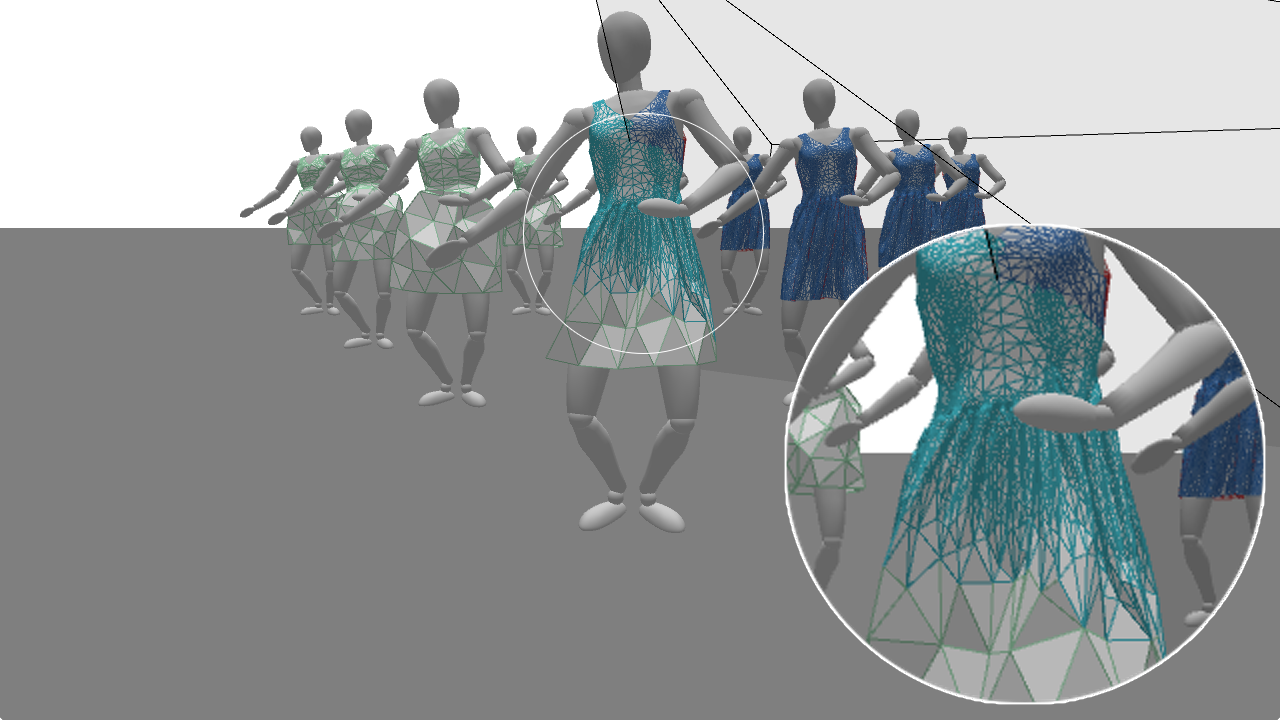
\includegraphics[width=1.0\columnwidth]{spatial_smoothing/spatial_smoothing}
	% \vspace*{-.15in}
    \caption{An example of spatial smoothing. Cyan edges indicate out-of-view faces
    under spatial smoothing, and green edges indicate out-of-view faces far from the view frustum.}
    \label{fig:spatial_smoothing}
	% \vspace*{-.2in}
\end{figure}

Instead of using a spatially discontinuous field, we enforce a continuous falloff of
the view factor between in-frame and out-of-frame faces. For a given mesh face,
let $d$ be its distance from the view frustum in world space. We define the
spatially smoothed view factor $\tilde\nu$ by linearly interpolating to $\nu_{\text{out}}$ over a user-specified margin length $m$:
\begin{align}
  \tilde\nu = \begin{cases}
    \nu_{\text{fb}} & \text{if $d = 0$}, \\
    \nu_{\text{fb}} - \frac dm(\nu_{\text{fb}} - \nu_{\text{out}}) & \text{if $0 < d < m$}, \\
    \nu_{\text{out}} & \text{if $d \ge m$},
  \end{cases}
\end{align}
where $\nu_{\text{fb}}$ is $1$ or $\nu_{\text{back}}$ depending on the direction of the face normal.
Thus, we have $\tilde\nu = 1$ or $\nu_{\text{back}}$ for visible faces and $\tilde\nu =
\nu_{\text{out}}$ for faces far from the view frustum, with a continuous transition region in between, as Figure \ref{fig:spatial_smoothing} shows.

There is still a discontinuity on the boundary between front-facing faces
and backward-facing faces. While it is tempting to use the direction of the
normal of back-faces to create a smooth transition, we find that normals can vary too
rapidly across silhouettes to offer any useful smoothing this way. Instead, we
address this discontinuity with a different approach, described later in
Section \ref{sec:silhouette-preserving}.

\subsubsection{Temporal smoothing and anticipation} 

We use temporal smoothing to avoid visibly discontinuous changes in mesh size due to camera motion, which
may cause noticeable popping artifacts. We include anticipation that ensures the
cloth gets refined to sufficient resolution \emph{before} it appears in the
frame, preventing undesirable transients.

% \begin{figure}[t]
%     \centering
%     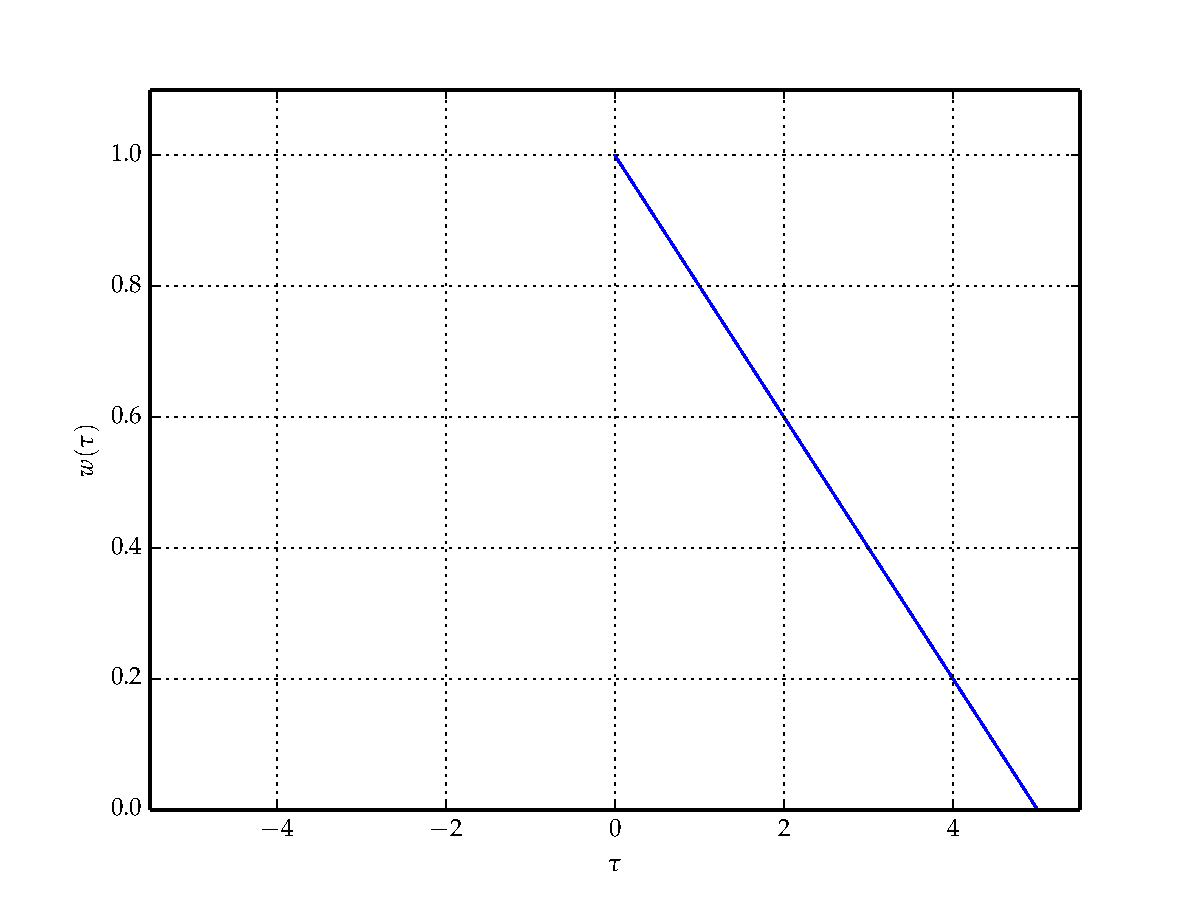
\includegraphics[width=1.0\columnwidth]{window_function}
%     \caption{A window function $w(\tau)$ when $T = 5$.}
%     \label{fig:window_function}
% \end{figure}

For any given face, we can treat the view factor before temporal smoothing $\tilde\nu$ as a function of time, holding the face fixed and considering the prescribed motion of the viewpoint.
We smooth $\tilde\nu$ over a time interval $[t,t+T]$ based on the current time $t$ as follows.
Define a temporal window function $w(\tau)$ which satisfies $w(0) = 1$ and falls off to zero at $\tau = T$.
The temporally smoothed view factor is
\begin{equation}
    \nu(t) = \max_{\tau\in[0,T]} w(\tau)\tilde\nu(t+\tau).
\end{equation}
% as illustrated in Figure \ref{fig:window_function}.
This is analogous to dilation by a non-flat structuring element in mathematical morphology.
In our implementation, we take $w(\tau) = 1 - \tau/T$.

\begin{figure}[t]
    \centering
    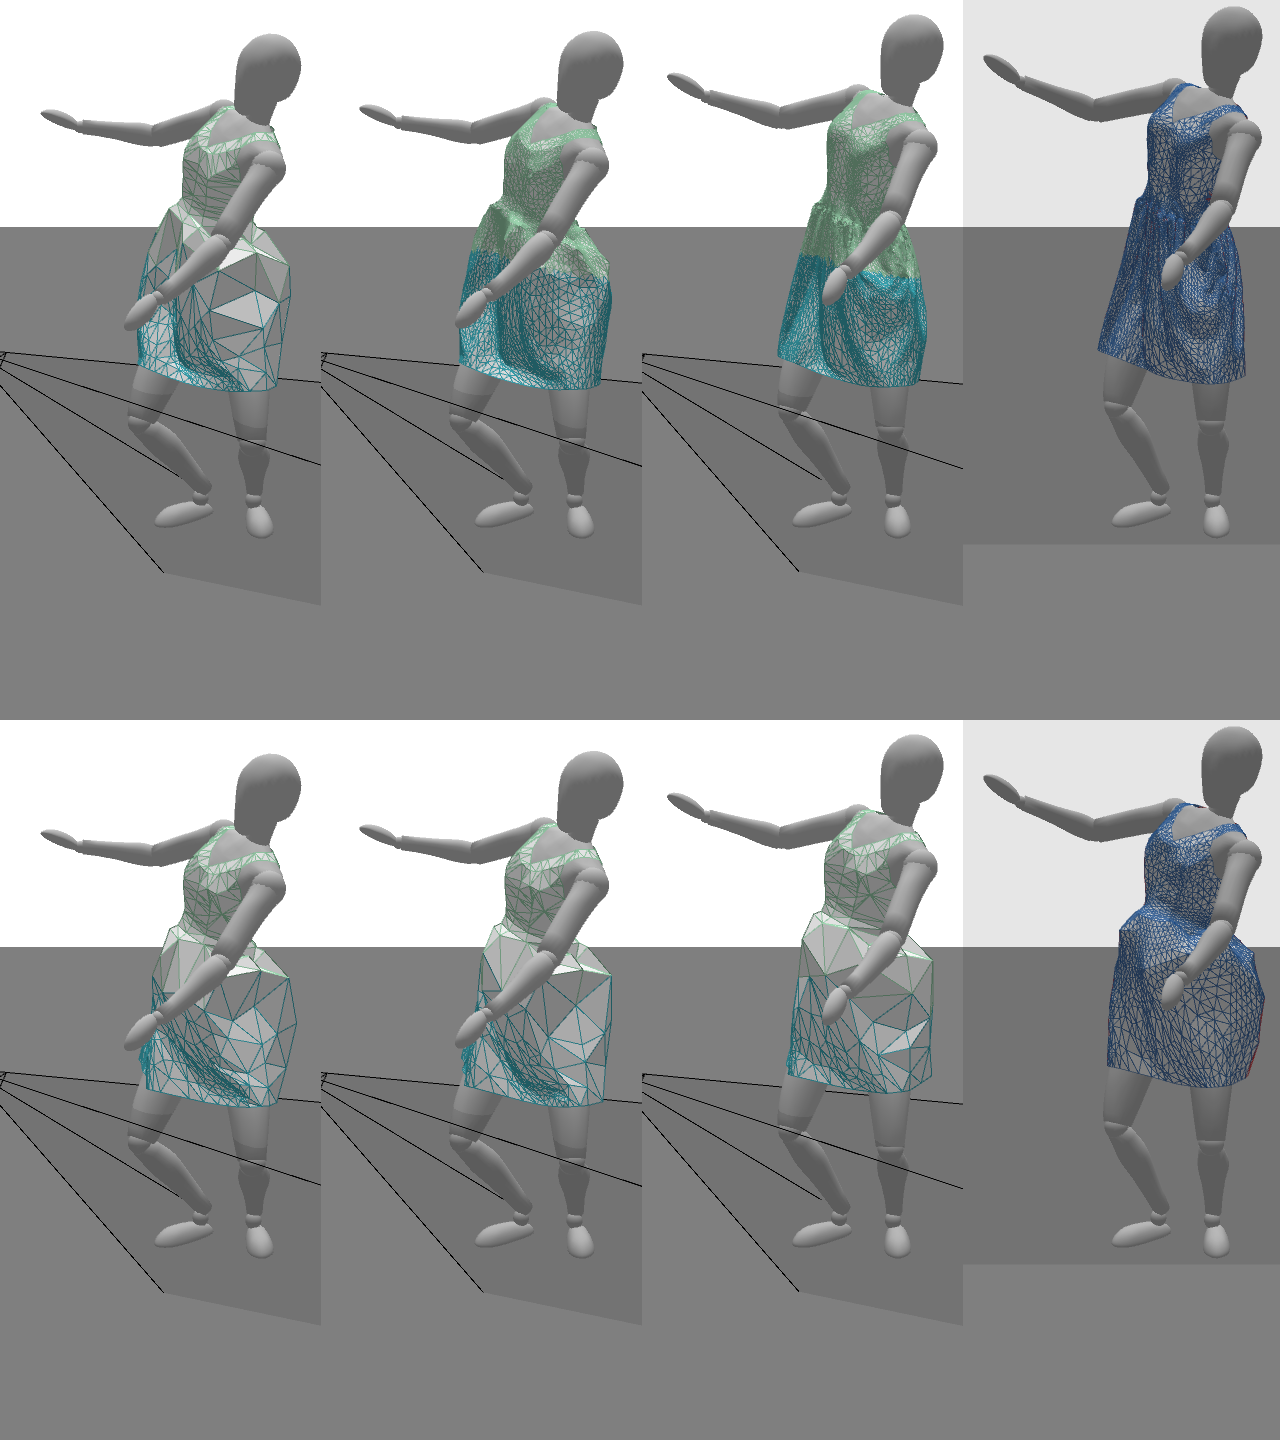
\includegraphics[width=1.0\columnwidth]{temporal_anticipation/temporal_anticipation}
	% \vspace*{-.15in}	
    \caption{A sequence of frames with a jump cut, showing a dress simulated with temporal anticipation (above), and without (below). Blue edges indicate faces visible in the current view. Temporal anticipation allows the cloth to reach the correct high-resolution state before it becomes visible.}
    \label{fig:temporal_anticipation}
	% \vspace*{-.2in}
\end{figure}

Unlike smoothing by, say, moving averages, our approach is conservative in that $\nu(t) \ge \tilde\nu(t)$; in particular, visible regions always have $\nu = 1$.
Further, in the presence of discontinuities such as jump cuts, $\nu$ increases continuously from $\nu_{\text{out}}$ to $1$ over a time period $T$ in advance of the jump.
This anticipatory refinement allows enough time for the system to settle into a feasible high-resolution state before becoming visible, as shown in Figure \ref{fig:temporal_anticipation}.

\subsection{Screen-space resolution of visible regions}

In non-visible regions, it is sufficient to uniformly coarsen the mesh resolution as above.
However, for visible regions, we wish to preserve the geometrical and dynamical detail resolved by the original sizing field as much as possible, only coarsening when such detail would not be visually important.

Our objective is that faces and edges in visible regions should be large enough to affect the visual appearance of cloth in the final image.
The farther a face is from a camera, the smaller it appears under perspective projection.
The projected area of a triangle also becomes smaller as the face normal becomes perpendicular to the viewing direction.
Therefore, in regions that are distant, or are not normal to the view direction, a high-resolution mesh will be wasteful as any detailed features resolved by the fine elements will appear extremely small in the final image.

In this section, we describe how to limit the refinement of mesh elements based on their projected sizes in screen space.
We do so by constraining the allowed edge lengths to a specified minimum visual angle in screen space.
This approach takes both orientation and depth into account in unified and consistent way.
Previous work~\cite{Narain:2012:AAR} constrains the allowed edge lengths in material space to a range $[\ell_{\min},\ell_{\max}]$ by clamping the eigenvalues of the sizing tensor to lie between $\ell_{\max}^{-2}$ and $\ell_{\min}^{-2}$.
In our work, however, we constrain the sizing tensor with respect to screen space rather than material space.
We transform the sizing tensor $\mathbf{M}_{\text{vd}}$ to screen space, apply the bound on the shortest allowable edge length, and
transform it back to material space.

For a given configuration of the sheet, consider the function from material-space coordinates of vertices to their screen-space coordinates.
On visible faces, this function is locally invertible and its Jacobian $\mathbf S$ is a full-rank $2\times2$ matrix that can be evaluated locally for each face.
As the sizing tensor $\mathbf M_{\text{vd}}$ acts as a quadratic form acting on vectors in material space, the corresponding tensor that acts on screen-space vectors can be obtained via the transformation
\begin{equation}
    \mathcal{S}(\mathbf{M}_{\text{vd}}) = \mathbf{S}^{-\mathsf T}\mathbf{M}_{\text{vd}}\mathbf{S}^{-1}.
\end{equation}

% To limit the refinement of mesh edges in screen space, we seek the tensor nearest to $\tilde{\mathbf M}_{\text{vd}} = \mathcal S(\mathbf M_{\text{vd}})$ so that screen-space edges of length $\ell_{\min}$ are allowed.\woojong{I feel this sentence is a little bit awkward.}
We seek the minimum change to the screen-space sizing tensor $\tilde{\mathbf M}_{\text{vd}} = \mathcal S(\mathbf M_{\text{vd}})$ such that edges of screen-space length $\ell_{\min}$ will not be refined further.
This modification can be achieved by clamping the eigenvalues of $\tilde{\mathbf M}_{\text{vd}}$ to not exceed $\ell^{-2}_{\min}$:
\begin{align}
  \tilde{\mathbf{M}}_{\text{vd}} &= \mathbf{Q}\begin{bmatrix}\tilde\lambda_1 & 0 \\ 0 & \tilde\lambda_2\end{bmatrix}\mathbf{Q}^{\mathsf T}, \\
  \hat\lambda_i &= \min(\tilde{\lambda}_i, \ell^{-2}_{\min}), \\
  \hat{\mathbf{M}}_{\text{vd}} &= \mathbf{Q}\begin{bmatrix}\hat\lambda_1 & 0 \\ 0 & \hat\lambda_2\end{bmatrix}\mathbf{Q}^{\mathsf T}.
\end{align}
We transform this modified screen-space tensor back into material space to
obtain the final sizing field we use for remeshing, $\mathcal
S^{-1}(\hat{\mathbf{M}}_{\text{vd}}) = \mathbf S^{\mathsf T}\hat{\mathbf
M}_{\text{vd}}\mathbf S$.


\subsection{Transferring sizing field from faces to vertices}
\label{sec:silhouette-preserving}

\begin{figure}[t]
    \centering
    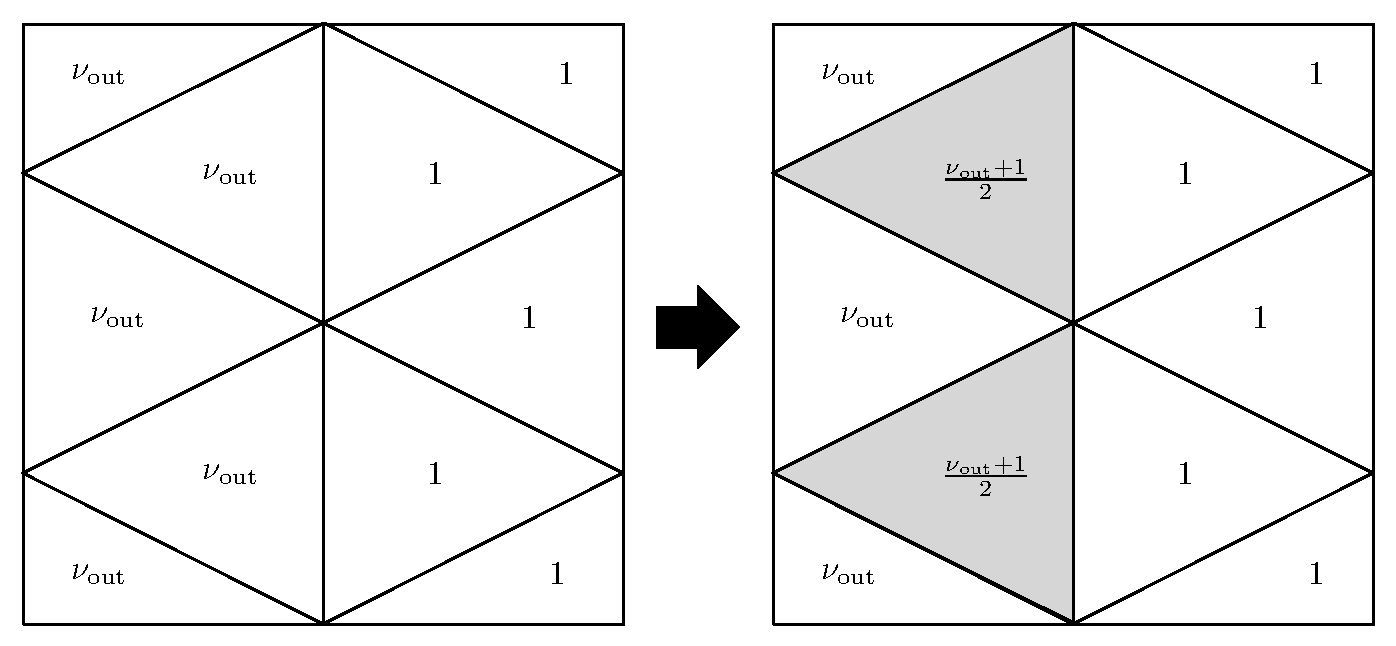
\includegraphics[width=0.8\columnwidth]{silhouette_preserving}
        % \vspace*{-.1in}
    \caption{Locally interpolating discontinuous view factors at silhouettes to ensure smooth silhouettes.}
    \label{fig:silhouette_preserving}
	% \vspace*{-.25in}
\end{figure}

The sizing field defined by the procedure above is represented as a tensor on each face.
This tensor field must be resampled onto mesh vertices so that it can be used in the sizing criterion
\eqref{eq:invalid}.  Previous work \cite{Narain:2012:AAR} has used a simple area-weighted
averaging procedure. However, we have found that that approach tends to lose detail in
regions with rapid variation in the sizing field, such as at silhouettes where the view
factor changes from $1$ to $\nu_{\text{out}}$. The issue is exacerbated because coarser
regions, which have larger faces, are given higher weight, leading to excessive coarsening
at boundary vertices.

In order to handle this discontinuity on view factors, we first resample per-face view
factors before the simple area-weighted averaging procedure. If the values of $\nu$ differ by more than a specified threshold across any edge, we do simple
averaging between two adjacent view factors, and assign the averaged value to one
of the faces as shown in Figure~\ref{fig:silhouette_preserving}. As we don't want to
change the view factors of the visible faces from $1$, we always assign the
averaged view factor to a non-visible face.
% \rahul{This is again like morphological dilation.}

This approach ensures that silhouette boundaries are refined to the same extent
as other visible regions of the cloth, improving the appearance of silhouettes.
This change affects the simulation mesh only in a limited area near silhouette
boundaries, so it does not hinder overall performance.

\subsection{Interpenetration handling}

Remeshing invariably produces changes in the geometry of the cloth mesh, and can introduce interpenetrations of the cloth with itself or with obstacles.
We found that the simple approach for interpenetration handling used in previous remeshing work \cite{Narain:2012:AAR} does not always converge to an interpenetration-free configuration in the presence of the agressive coarsening we perform in non-visible regions.
Instead we use the approach of intersection contour minimization proposed by Volino et al.~\cite{Volino:2006:RSC}, which we found to be robust to large and complex interpenetrations.

\section{Results and Discussion}

\begin{figure}[t]
    \centering
    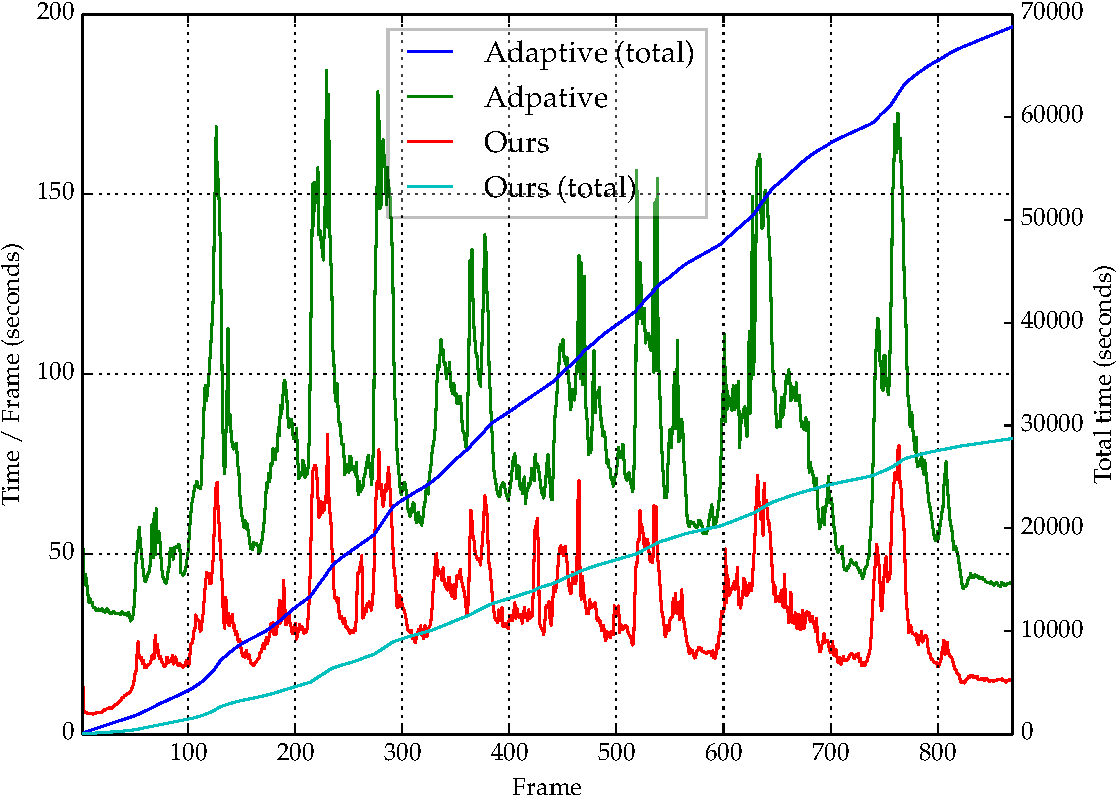
\includegraphics[width=1.0\columnwidth]{timings}
	% \vspace*{-.15in}	
    \caption{A comparison of view-independent and view-dependent adaptive simulations for
        the example of Figure \ref{fig:teaser} in terms of per-frame and cumulative simulation times.}
    \label{fig:comparison}
	% \vspace*{-.2in}
\end{figure}

\begin{figure}[t]
    \centering
    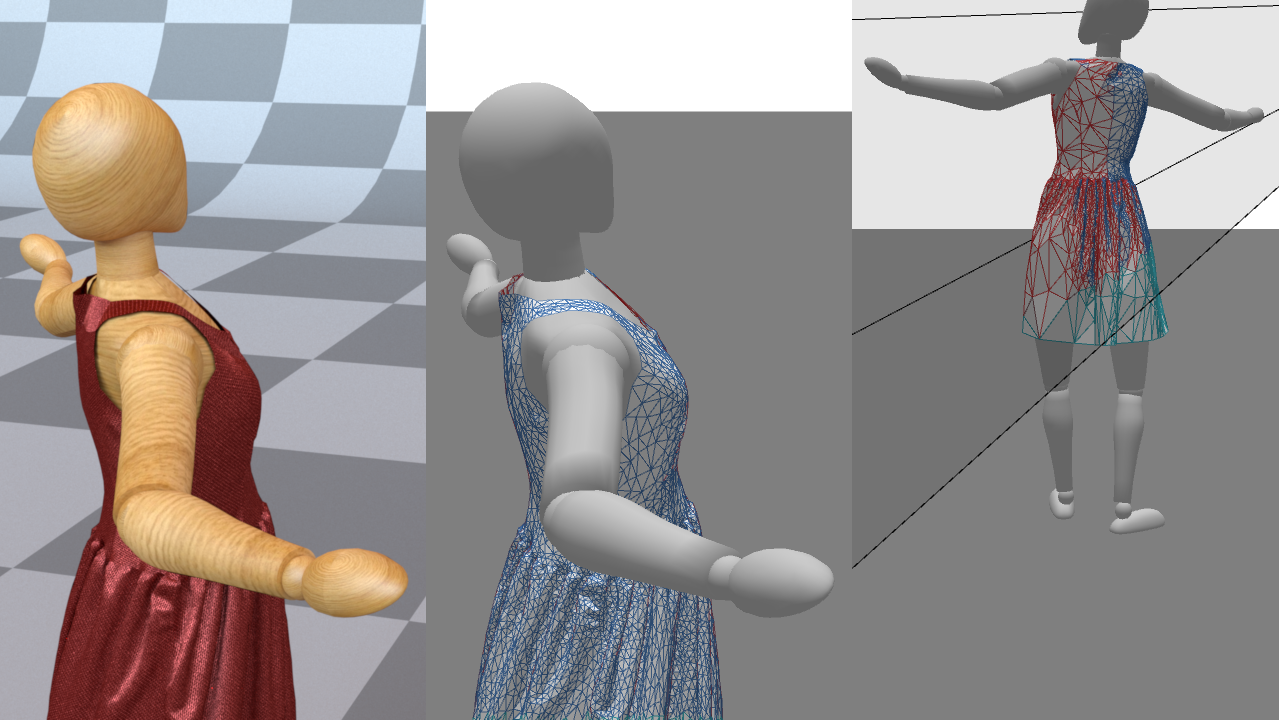
\includegraphics[width=1.0\columnwidth]{solo/solo}
	% \vspace*{-.15in}	
    \caption{A solo dancer is shown from the camera's perspective (left, middle) and from
    an external perspective with the camera's view frustum drawn in black wireframe (right).}
    \label{fig:solo_dancer}
	% \vspace*{-.2in}
\end{figure}

\begin{figure}[t]
    \centering
    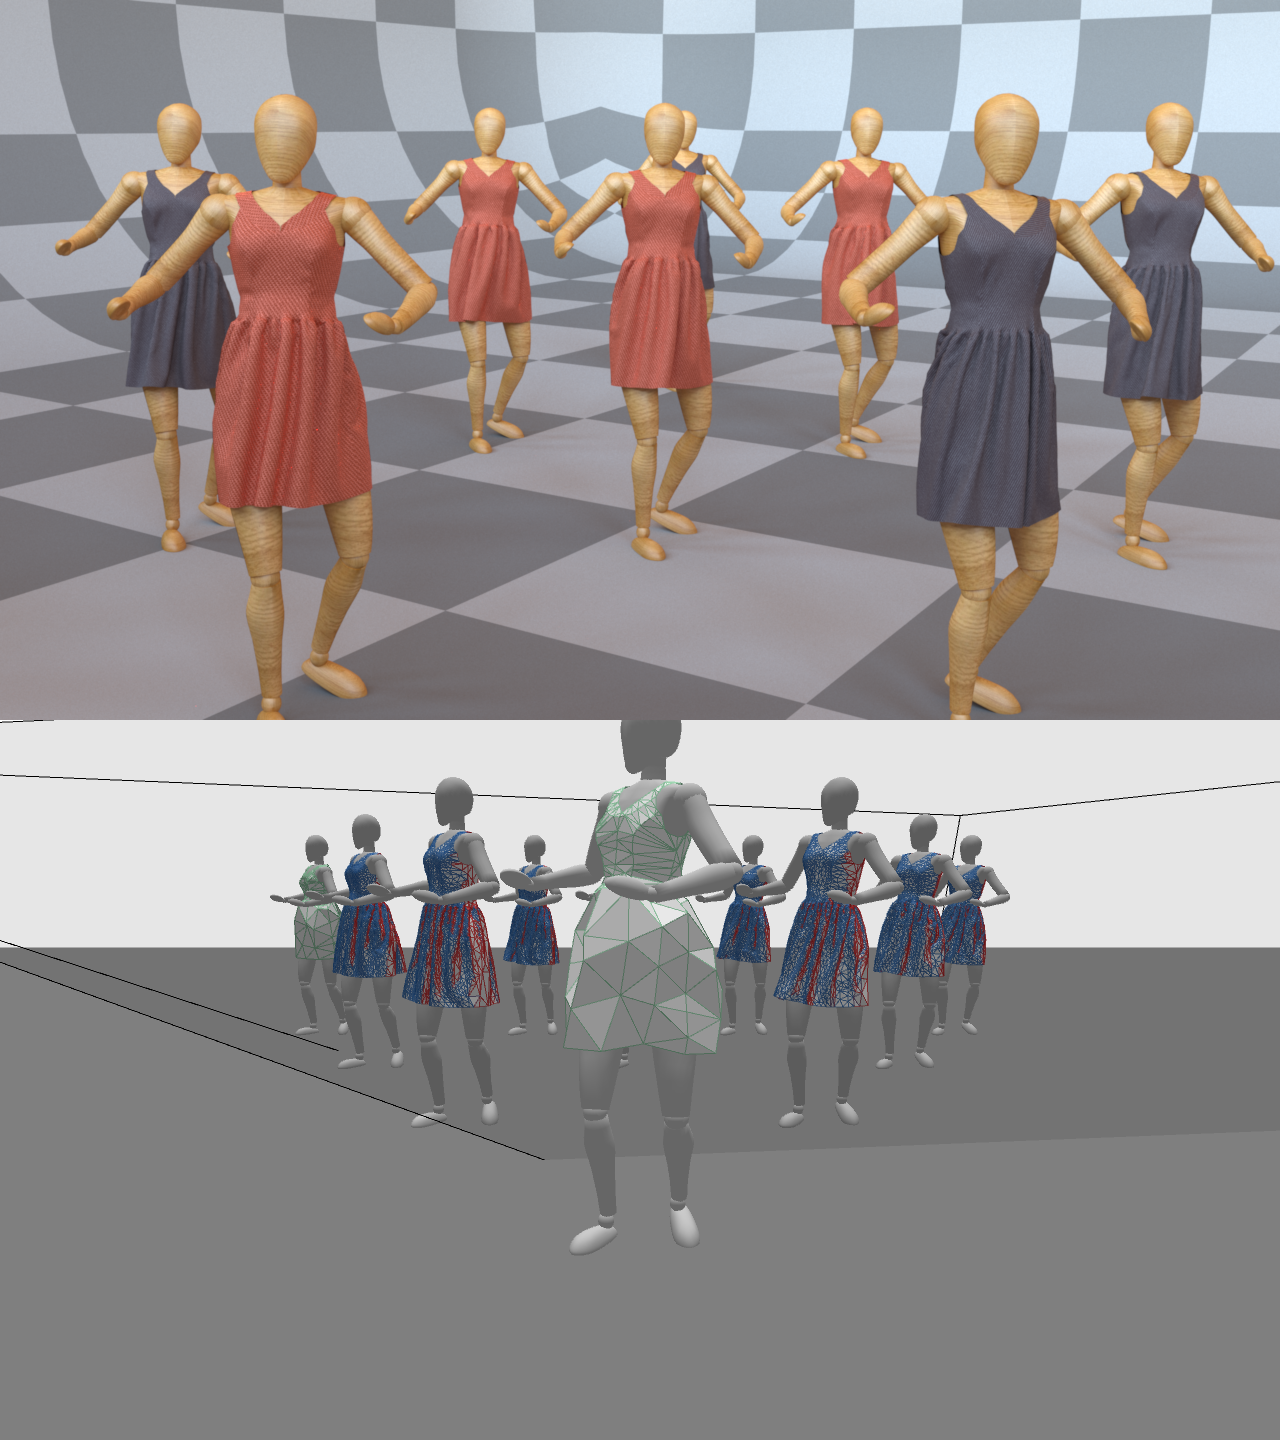
\includegraphics[width=1.0\columnwidth]{crowd/crowd}
	% \vspace*{-.15in}	
    \caption{A group of multiple dancers is rendered from the camera's perspective (top), while 
	an external view showing the camera's view frustum is shown below. Characters
      completely outside the view frustum are simulated at very low resolution.}
    \label{fig:crowd}
	% \vspace*{-.2in}
\end{figure}

\begin{table*}[t]
    \centering
    \resizebox{\textwidth}{!}{\begin{tabular}{l|rrr|rrr|rrr|r}  %modified
\toprule
{} & \multicolumn{3}{c|}{Num. Faces} & \multicolumn{3}{c|}{Num. Vertices} & \multicolumn{3}{c|}{Time / Frame (seconds)} & Speed-up\\  %modified
{} & min & max & mean & min & max & mean & min & max &  mean & {}\\ %modified
\hline
Karate&&&&&&&&&&\\
~~~Non-adaptive   & 123,790 & 123,790 & 123,790 &  63,889 &  63,889 &  63,889 & 136.47 & 288.01 & 161.44 & 0.49$\times$\\
~~~Adaptive       &  25,785 &  71,142 &  41,973 &  14,135 &  37,199 &  22,358 &  31.41 & 184.39 &  79.04 &    1$\times$\\
~~~View-dependent &   5,223 &  39,139 &  21,501 &   3,142 &  20,770 &  11,670 &   5.52 &  83.29 &  33.02 & 2.39$\times$ \\[0.2cm]  %vertical gap
Solo Dancer &&&&&&&&&&\\
~~~Non-adaptive   &  43,710 &  43,710 &  43,710 &  22,736 &  22,736 &  22,736 &  27.31 &  58.09 &  29.27 & 0.54$\times$\\
~~~Adaptive       &  12,030 &  21,763 &  18,041 &   6,593 &  11,535 &   9,659 &   7.78 &  22.00 &  15.80 &    1$\times$\\
~~~View-dependent &     730 &  15,951 &   9,638 &     560 &   8,599 &   5,314 &   0.83 &  13.81 &   7.55 & 2.09$\times$ \\[0.2cm]  %vertical gap
Multiple Dancers &&&&&&&&&&\\
~~~Non-adaptive   & 437,100 & 437,100 & 437,100 & 227,360 & 227,360 & 227,360 & 273.13 & 580.85 & 292.73 & 0.47$\times$\\
~~~Adaptive       & 119,515 & 184,340 & 161,028 &  65,505 &  98,630 &  86,897 &  79.97 & 178.24 & 136.99 &    1$\times$\\
~~~View-dependent &  11,216 & 102,945 &  36,339 &   7,619 &  56,285 &  21,228 &  12.02 &  82.54 &  30.76 & 4.45$\times$\\
\bottomrule
\end{tabular}
}
    \caption{Statistics and timing numbers for the examples. Non-adaptive simulations use a fixed
    high-resolution mesh. 
	Adaptive simulations use the unmodified scheme implemented in ARCSim. % Times doesn't do italic small-caps
	View-dependent simulations use the method described in this paper.
	The adaptive simulations are used as a baseline for comparison.  
	The non-adaptive mesh resolution was selected to match the visual quality of the 
	adaptive simulations.
}
\label{table:timings}
	% \vspace*{-.2in}
\end{table*}


We have implemented the methods described in this paper as an extension to the
\arcsim code. The code implementation will be published with this paper. To
test the utility of the proposed methods, we ran comparisons with adaptive and
non-adaptive simulations on several
examples. All simulations were run on a machine with an Intel Xeon E5-2680 v2
processor and 16 GB RAM using 4 execution threads.
The constants for view-dependent refinement that were used for these examples are
$\nu_{\text{back}} = 0.2$, $m = 0.4\ \mathrm{m}$, $T = 5\ \mathrm{frames}$, and
$\nu_{\text{out}} = 0.01$.  For the example shown in Figure 1, we used larger
$\nu_{\text{out}} = 0.1$ to avoid intersection problems with the layered garments.

Figure~\ref{fig:teaser} shows a character wearing a layered outfit consisting
of three interacting garments. As the accompanying video shows, the
character's clothing exhibits complex dynamic motion with detailed wrinkles. As
the camera moves continuously or transits between cuts, the simulation mesh
is updated to maintain a constant level of visible detail while out-of-view
regions are aggressively coarsened. Figure~\ref{fig:comparison} plots the time
per frame and total cumulative computation time for this example for both the
basic adaptive simulation and the view-dependent version.

Figure~\ref{fig:solo_dancer} shows a character wearing a simple
dress, showing a similar degree of view-dependent refinement and coarsening to Figure~\ref{fig:teaser}.
A group of ten such characters is shown in
Figure~\ref{fig:crowd}. Note that while these characters are all
performing the same actions in the same type of dress, they are simulated individually
with different resolutions depending on their location relative to the viewpoint.
In practical applications, multiple characters in a crowd
would have different garments and motions and would therefore have to be simulated
individually even without view dependence.

Timings for these three examples are reported in Table~\ref{table:timings}. The single characters
realize a speed-up between $2.1\times$ and $2.4\times$. This speed-up becomes
more substantial for the group of ten characters where it is roughly
$4.5\times$. The greater speed-up occurs because when a single character fills
the screen, requiring full adaptive resolution, it tends to obscure others
which then switch to low resolution and generate substantial savings. In order
for all characters to be visible, the camera must be fairly far back which
yields savings across all characters. These observations would hold more
strongly for larger groups. Accordingly we hypothesize that massive scenes
involving thousands of characters would likely realize speed-up substantially
larger than those we have observed for small groups.

% Figures~\ref{fig:temporal_anticipation} and~\ref{fig:spatial_smoothing}
% illustrate how refinement is extended in time and space. This extension keeps
% the unphysical motion induced by aggressive resolution changes outside the
% visible region.

Remeshing does introduce small amounts of motion that might be visible if
the character is otherwise still. As shown in the video, however, this motion
does not manifest as visible popping because the dramatic remeshing generally
happens off screen. The motion that appears on screen is gentle swaying that
looks fairly natural. If the subject is moving, then the artificial motion is
completely masked by the normal motion of the cloth. Even with a still subject, the
artificial motion can be hard to detect due to the movement of the camera.


\section{Conclusions}

The methods we have described provide a simple way of achieving computational
savings for cloth simulation. For scenes involving multiple characters or large
crowds, these savings can be substantial. We have demonstrated our approach in
simulations of clothing, but believe that it could equally well be applied to
other objects that can be simulated in an adaptive framework, including
materials that can crumple\cite{Narain:2013:FCA} or
fracture\cite{Pfaff:2014:ATC}.

The main limitation of our method is that it requires an adaptive framework.
However, once that framework is in place, view-dependent adaptivity is
relatively simple to implement. For the group of dancers, our view-dependent adaptive
simlation is nearly ten times faster than non-adaptive simulation. We
believe that such large performance gains outweigh any costs associated
with changing mesh topology. We also believe that our approach
would scale very well to massive scenes with thousands of actors, where it would
produce even larger savings.


In general, simulations used for physically based animation in
graphics have been designed so that they capture visible phenomena for
realistic appearance.  These simulations typically avoid the type of
error analysis that one finds in most engineering contexts because it
is difficult to quantify a measure of perceptual error that would be
relevant to graphics simulations.  The work we've presented here
explicitly drives adaption according to a heuristic measure of visible
error.  Future work in this area could more explicitly
take perceptual error into account so that reduced resolution could be
used where masking effects due to motion, complexity, or other
phenomena cause humans to be less sensitive to apparent detail.



%\section*{Acknowledgments}
% <<>> Removed for anonymous review.


%----------------------------------------------------------------------------
%----------------------------------------------------------------------------

\bibliographystyle{TexInputs/eg-alpha-doi}
\bibliography{viewdep-paper}

%----------------------------------------------------------------------------
%----------------------------------------------------------------------------


\end{document}

% LocalWords:  anisotropic
